\documentclass{scrartcl}
\usepackage{mathtools}
\usepackage{tikz}
\usetikzlibrary{trees,positioning}

\begin{document}
\begin{figure}
\centering
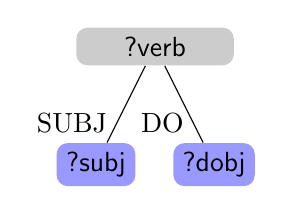
\begin{tikzpicture}
\node[fill = gray!40, shape = rectangle, rounded corners, minimum width = 2cm, font = \sffamily] (28) {?verb}
child {node[fill = blue!40, shape = rectangle, rounded corners, minimum width = 1cm, font = \sffamily]  (29) {?subj}
}
child {node[fill = blue!40, shape = rectangle, rounded corners, minimum width = 1cm, font = \sffamily]  (30) {?dobj}
}
;
\begin{scope}[nodes = {draw = none}]
\path (29)     -- (28) node [near start, left]  {\text{SUBJ}};
\path (30)     -- (28) node [near start, left]  {\text{DO}};
\draw[densely dashed, rounded corners, thin];
\end{scope} 
\end{tikzpicture}
\caption{Visualisation for SPARQLPattern\_ES\_1}
\label{fig:SPARQLPatternES1}
\end{figure}


\begin{figure}
\centering
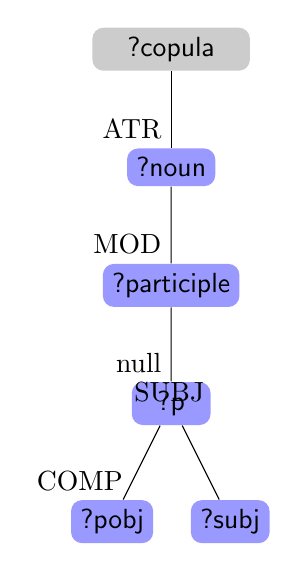
\begin{tikzpicture}
\node[fill = gray!40, shape = rectangle, rounded corners, minimum width = 2cm, font = \sffamily] (30) {?copula}
child {node[fill = blue!40, shape = rectangle, rounded corners, minimum width = 1cm, font = \sffamily]  (31) {?noun}
child {node[fill = blue!40, shape = rectangle, rounded corners, minimum width = 1cm, font = \sffamily] (32) {?participle}
child {node[fill = blue!40, shape = rectangle, rounded corners, minimum width = 1cm, font = \sffamily] (33) {?p}
child {node[fill = blue!40, shape = rectangle, rounded corners, minimum width = 1cm, font = \sffamily] (34) {?pobj}
}
child {node[fill = blue!40, shape = rectangle, rounded corners, minimum width = 1cm, font = \sffamily]  (35) {?subj}
}
}}};
\begin{scope}[nodes = {draw = none}]
\path (31)     -- (30) node [near start, left]  {\text{ATR}};
\path (32)     -- (31) node [near start, left]  {\text{MOD}};
\path (33)     -- (32) node [near start, left]  {\text{null}};
\path (35)     -- (30) node [near start, left]  {\text{SUBJ}};
\path (34)     -- (33) node [near start, left]  {\text{COMP}};
\draw[densely dashed, rounded corners, thin];
\end{scope} 
\end{tikzpicture}
\caption{Visualisation for SPARQLPattern\_ES\_2}
\label{fig:SPARQLPatternES2}
\end{figure}


\begin{figure}
\centering
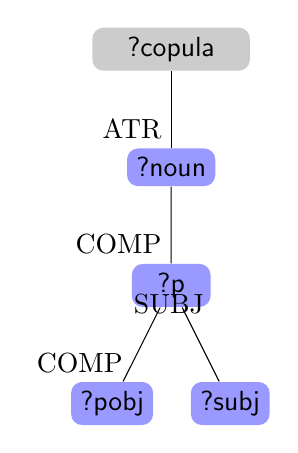
\begin{tikzpicture}
\node[fill = gray!40, shape = rectangle, rounded corners, minimum width = 2cm, font = \sffamily] (35) {?copula}
child {node[fill = blue!40, shape = rectangle, rounded corners, minimum width = 1cm, font = \sffamily]  (36) {?noun}
child {node[fill = blue!40, shape = rectangle, rounded corners, minimum width = 1cm, font = \sffamily] (37) {?p}
child {node[fill = blue!40, shape = rectangle, rounded corners, minimum width = 1cm, font = \sffamily] (38) {?pobj}
}
child {node[fill = blue!40, shape = rectangle, rounded corners, minimum width = 1cm, font = \sffamily]  (39) {?subj}
}
}};
\begin{scope}[nodes = {draw = none}]
\path (36)     -- (35) node [near start, left]  {\text{ATR}};
\path (37)     -- (36) node [near start, left]  {\text{COMP}};
\path (39)     -- (35) node [near start, left]  {\text{SUBJ}};
\path (38)     -- (37) node [near start, left]  {\text{COMP}};
\draw[densely dashed, rounded corners, thin];
\end{scope} 
\end{tikzpicture}
\caption{Visualisation for SPARQLPattern\_ES\_2b}
\label{fig:SPARQLPatternES2b}
\end{figure}


\begin{figure}
\centering
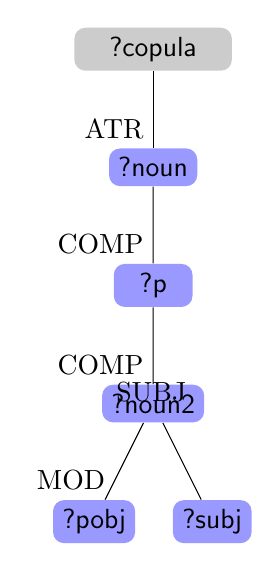
\begin{tikzpicture}
\node[fill = gray!40, shape = rectangle, rounded corners, minimum width = 2cm, font = \sffamily] (39) {?copula}
child {node[fill = blue!40, shape = rectangle, rounded corners, minimum width = 1cm, font = \sffamily]  (40) {?noun}
child {node[fill = blue!40, shape = rectangle, rounded corners, minimum width = 1cm, font = \sffamily] (41) {?p}
child {node[fill = blue!40, shape = rectangle, rounded corners, minimum width = 1cm, font = \sffamily] (42) {?noun2}
child {node[fill = blue!40, shape = rectangle, rounded corners, minimum width = 1cm, font = \sffamily] (43) {?pobj}
}
child {node[fill = blue!40, shape = rectangle, rounded corners, minimum width = 1cm, font = \sffamily]  (44) {?subj}
}
}}};
\begin{scope}[nodes = {draw = none}]
\path (40)     -- (39) node [near start, left]  {\text{ATR}};
\path (41)     -- (40) node [near start, left]  {\text{COMP}};
\path (42)     -- (41) node [near start, left]  {\text{COMP}};
\path (44)     -- (39) node [near start, left]  {\text{SUBJ}};
\path (43)     -- (42) node [near start, left]  {\text{MOD}};
\draw[densely dashed, rounded corners, thin];
\end{scope} 
\end{tikzpicture}
\caption{Visualisation for SPARQLPattern\_ES\_2c}
\label{fig:SPARQLPatternES2c}
\end{figure}


null


\begin{figure}
\centering
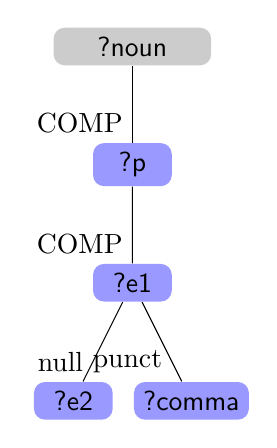
\begin{tikzpicture}
\node[fill = gray!40, shape = rectangle, rounded corners, minimum width = 2cm, font = \sffamily] (44) {?noun}
child {node[fill = blue!40, shape = rectangle, rounded corners, minimum width = 1cm, font = \sffamily]  (45) {?p}
child {node[fill = blue!40, shape = rectangle, rounded corners, minimum width = 1cm, font = \sffamily] (46) {?e1}
child {node[fill = blue!40, shape = rectangle, rounded corners, minimum width = 1cm, font = \sffamily] (47) {?e2}
}
child {node[fill = blue!40, shape = rectangle, rounded corners, minimum width = 1cm, font = \sffamily] (48) {?comma}
}
}};
\begin{scope}[nodes = {draw = none}]
\path (45)     -- (44) node [near start, left]  {\text{COMP}};
\path (46)     -- (45) node [near start, left]  {\text{COMP}};
\path (47)     -- (46) node [near start, left]  {\text{null}};
\path (48)     -- (46) node [near start, left]  {\text{punct}};
\draw[densely dashed, rounded corners, thin];
\end{scope} 
\end{tikzpicture}
\caption{Visualisation for SPARQLPattern\_ES\_4}
\label{fig:SPARQLPatternES4}
\end{figure}


\begin{figure}
\centering
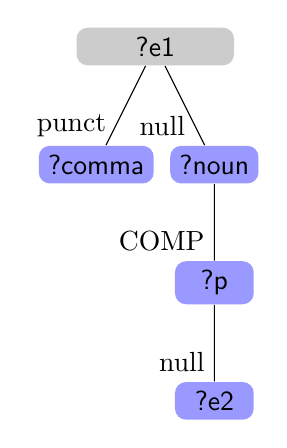
\begin{tikzpicture}
\node[fill = gray!40, shape = rectangle, rounded corners, minimum width = 2cm, font = \sffamily] (48) {?e1}
child {node[fill = blue!40, shape = rectangle, rounded corners, minimum width = 1cm, font = \sffamily]  (49) {?comma}
}
child {node[fill = blue!40, shape = rectangle, rounded corners, minimum width = 1cm, font = \sffamily]  (50) {?noun}
child {node[fill = blue!40, shape = rectangle, rounded corners, minimum width = 1cm, font = \sffamily] (51) {?p}
child {node[fill = blue!40, shape = rectangle, rounded corners, minimum width = 1cm, font = \sffamily] (52) {?e2}
}
}};
\begin{scope}[nodes = {draw = none}]
\path (49)     -- (48) node [near start, left]  {\text{punct}};
\path (50)     -- (48) node [near start, left]  {\text{null}};
\path (51)     -- (50) node [near start, left]  {\text{COMP}};
\path (52)     -- (51) node [near start, left]  {\text{null}};
\draw[densely dashed, rounded corners, thin];
\end{scope} 
\end{tikzpicture}
\caption{Visualisation for SPARQLPattern\_ES\_5}
\label{fig:SPARQLPatternES5}
\end{figure}


\begin{figure}
\centering
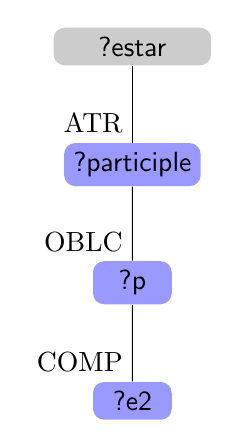
\begin{tikzpicture}
\node[fill = gray!40, shape = rectangle, rounded corners, minimum width = 2cm, font = \sffamily] (52) {?estar}
child {node[fill = blue!40, shape = rectangle, rounded corners, minimum width = 1cm, font = \sffamily]  (53) {?participle}
child {node[fill = blue!40, shape = rectangle, rounded corners, minimum width = 1cm, font = \sffamily] (54) {?p}
child {node[fill = blue!40, shape = rectangle, rounded corners, minimum width = 1cm, font = \sffamily] (55) {?e2}
}
}};
\begin{scope}[nodes = {draw = none}]
\path (53)     -- (52) node [near start, left]  {\text{ATR}};
\path (54)     -- (53) node [near start, left]  {\text{OBLC}};
\path (55)     -- (54) node [near start, left]  {\text{COMP}};
\draw[densely dashed, rounded corners, thin];
\end{scope} 
\end{tikzpicture}
\caption{Visualisation for SPARQLPattern\_ES\_6}
\label{fig:SPARQLPatternES6}
\end{figure}


\begin{figure}
\centering
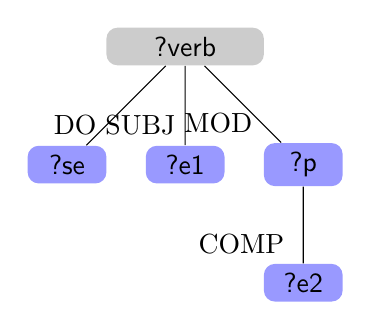
\begin{tikzpicture}
\node[fill = gray!40, shape = rectangle, rounded corners, minimum width = 2cm, font = \sffamily] (55) {?verb}
child {node[fill = blue!40, shape = rectangle, rounded corners, minimum width = 1cm, font = \sffamily]  (56) {?se}
}
child {node[fill = blue!40, shape = rectangle, rounded corners, minimum width = 1cm, font = \sffamily]  (57) {?e1}
}
child {node[fill = blue!40, shape = rectangle, rounded corners, minimum width = 1cm, font = \sffamily]  (58) {?p}
child {node[fill = blue!40, shape = rectangle, rounded corners, minimum width = 1cm, font = \sffamily] (59) {?e2}
}
};
\begin{scope}[nodes = {draw = none}]
\path (56)     -- (55) node [near start, left]  {\text{DO}};
\path (57)     -- (55) node [near start, left]  {\text{SUBJ}};
\path (58)     -- (55) node [near start, left]  {\text{MOD}};
\path (59)     -- (58) node [near start, left]  {\text{COMP }};
\draw[densely dashed, rounded corners, thin];
\end{scope} 
\end{tikzpicture}
\caption{Visualisation for SPARQLPattern\_ES\_7}
\label{fig:SPARQLPatternES7}
\end{figure}


\begin{figure}
\centering
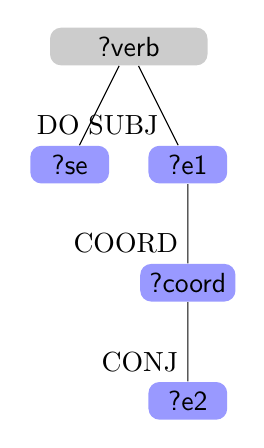
\begin{tikzpicture}
\node[fill = gray!40, shape = rectangle, rounded corners, minimum width = 2cm, font = \sffamily] (59) {?verb}
child {node[fill = blue!40, shape = rectangle, rounded corners, minimum width = 1cm, font = \sffamily]  (60) {?se}
}
child {node[fill = blue!40, shape = rectangle, rounded corners, minimum width = 1cm, font = \sffamily]  (61) {?e1}
child {node[fill = blue!40, shape = rectangle, rounded corners, minimum width = 1cm, font = \sffamily] (62) {?coord}
child {node[fill = blue!40, shape = rectangle, rounded corners, minimum width = 1cm, font = \sffamily] (63) {?e2}
}
}};
\begin{scope}[nodes = {draw = none}]
\path (60)     -- (59) node [near start, left]  {\text{DO}};
\path (61)     -- (59) node [near start, left]  {\text{SUBJ}};
\path (62)     -- (61) node [near start, left]  {\text{COORD}};
\path (63)     -- (62) node [near start, left]  {\text{CONJ}};
\draw[densely dashed, rounded corners, thin];
\end{scope} 
\end{tikzpicture}
\caption{Visualisation for SPARQLPattern\_ES\_7b}
\label{fig:SPARQLPatternES7b}
\end{figure}


\begin{figure}
\centering
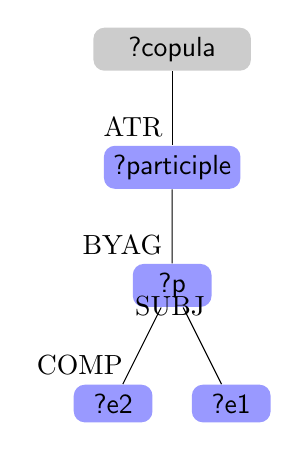
\begin{tikzpicture}
\node[fill = gray!40, shape = rectangle, rounded corners, minimum width = 2cm, font = \sffamily] (63) {?copula}
child {node[fill = blue!40, shape = rectangle, rounded corners, minimum width = 1cm, font = \sffamily]  (64) {?participle}
child {node[fill = blue!40, shape = rectangle, rounded corners, minimum width = 1cm, font = \sffamily] (65) {?p}
child {node[fill = blue!40, shape = rectangle, rounded corners, minimum width = 1cm, font = \sffamily] (66) {?e2}
}
child {node[fill = blue!40, shape = rectangle, rounded corners, minimum width = 1cm, font = \sffamily]  (67) {?e1}
}
}};
\begin{scope}[nodes = {draw = none}]
\path (64)     -- (63) node [near start, left]  {\text{ATR}};
\path (67)     -- (63) node [near start, left]  {\text{SUBJ}};
\path (65)     -- (64) node [near start, left]  {\text{BYAG}};
\path (66)     -- (65) node [near start, left]  {\text{COMP}};
\draw[densely dashed, rounded corners, thin];
\end{scope} 
\end{tikzpicture}
\caption{Visualisation for SPARQLPattern\_ES\_8}
\label{fig:SPARQLPatternES8}
\end{figure}


\begin{figure}
\centering
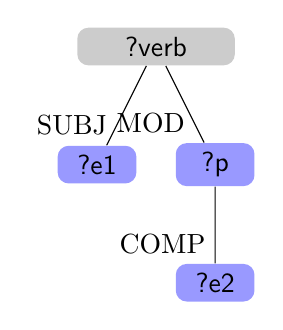
\begin{tikzpicture}
\node[fill = gray!40, shape = rectangle, rounded corners, minimum width = 2cm, font = \sffamily] (67) {?verb}
child {node[fill = blue!40, shape = rectangle, rounded corners, minimum width = 1cm, font = \sffamily]  (68) {?e1}
}
child {node[fill = blue!40, shape = rectangle, rounded corners, minimum width = 1cm, font = \sffamily]  (69) {?p}
child {node[fill = blue!40, shape = rectangle, rounded corners, minimum width = 1cm, font = \sffamily] (70) {?e2}
}
};
\begin{scope}[nodes = {draw = none}]
\path (68)     -- (67) node [near start, left]  {\text{SUBJ}};
\path (69)     -- (67) node [near start, left]  {\text{MOD}};
\path (70)     -- (69) node [near start, left]  {\text{COMP}};
\draw[densely dashed, rounded corners, thin];
\end{scope} 
\end{tikzpicture}
\caption{Visualisation for SPARQLPattern\_ES\_9}
\label{fig:SPARQLPatternES9}
\end{figure}


\end{document}